\documentclass[14pt]{beamer} %Makes presentation
%\documentclass[handout]{beamer} %Makes Handouts
\usetheme{Singapore} %Gray with fade at top
\useoutertheme[subsection=false]{miniframes} %Supppress subsection in header
\useinnertheme{rectangles} %Itemize/Enumerate boxes
\usecolortheme{seagull} %Color theme
\usecolortheme{rose} %Inner color theme

\definecolor{light-gray}{gray}{0.75}
\definecolor{dark-gray}{gray}{0.55}
\setbeamercolor{item}{fg=light-gray}
\setbeamercolor{enumerate item}{fg=dark-gray}

\setbeamertemplate{navigation symbols}{}
%\setbeamertemplate{mini frames}[default]
\setbeamercovered{dynamics}
\setbeamerfont*{title}{size=\Large,series=\bfseries}

%\setbeameroption{notes on second screen} %Dual-Screen Notes
%\setbeameroption{show only notes} %Notes Output

\setbeamertemplate{frametitle}{\vspace{.5em}\bfseries\insertframetitle}
\newcommand{\heading}[1]{\noindent \textbf{#1}\\ \vspace{1em}}

\usepackage{bbding,color,multirow,times,ccaption,tabularx,graphicx,verbatim,booktabs,fixltx2e}
\usepackage{colortbl} %Table overlays
\usepackage[english]{babel}
\usepackage[latin1]{inputenc}
\usepackage[T1]{fontenc}
\usepackage{lmodern}

%\author[]{Thomas J. Leeper}
\institute[]{
  \inst{}%
  Department of Political Science and Government\\Aarhus University
}

\usepackage{tikz}
\usetikzlibrary{shapes,arrows}
\usetikzlibrary{decorations.pathreplacing}

\title{Research Designs for Causal Inference}

\date[]{March 10, 2015}

\begin{document}

\frame{\titlepage}

\frame{\tableofcontents}

\section{Background}

\frame{
	\frametitle{Background}
	\begin{itemize}\itemsep1.5em
		\item The experimental ideal!
		\item All observational studies require an \textbf{identification strategy}
		\item We've been focusing on conditioning (via matching and/or regression)
		\item Today's lecture is about quasi-experimental designs
	\end{itemize}
}

\frame{
	\frametitle{What is a Quasi-Experiment?}
	\begin{itemize}\itemsep1em
		\item<1-> A situation where a real-world event induces an exogenous change (or ``shock'') in an independent variable
		\item<2-> Also sometimes called \textit{``natural'' experiments}
		\item<3-> Can anyone think of examples?
	\end{itemize}
}

\frame{
	\frametitle{Design Trumps Analysis}
	\begin{itemize}\itemsep2em
		\item Observational studies are hard because we need to have a convincing causal theory and have observed all causally relevant variables
		\item Quasi-Experiments potentially save us from needing a complete and fully observed set of causal variables
		\item In a quasi-experiment, we can treat our data (almost) as-if they are from an experiment
	\end{itemize}
}

\section[IV]{Instrumental Variables}
\frame{\tableofcontents[currentsection]}

\frame{
	\frametitle{A little history}
	\begin{itemize}\itemsep1em
		\item Have been used for a very long time (since Wright 1928)
		\item Very popular identification strategy in economics
		\item Just starting to become widespread in political science
	\end{itemize}
}

\frame{
	\frametitle{When would we use IV?}
	\begin{itemize}\itemsep1em
		\item We are interested in the effect of $X \rightarrow Y$
		\item This relationship is confounded by unobservables
		\item We cannot manipulate $X$ (i.e., no experiments)
		\item How can we identify the effect $X \rightarrow Y$?
	\end{itemize}
}

\frame{
	\begin{center}
		\begin{tikzpicture}[>=latex',circ/.style={draw, shape=circle, node distance=5cm, line width=1.5pt}]
		\draw[->] (0,0) node[left] (X) {X} -- (5,0) node[right] (Y) {Y};
		\draw[->] (-3,4) node[above] (Z) {Z} -- (X);
		\draw[->] (Z) -- (Y);
		\draw[->] (5,2) node[above] (A) {A} -- (Y);
		\draw<1>[->] (-2,0) node[left] (B) {B} -- (X);
		\draw<2>[->,red,thick] (-2,0) node[left] (B) {\color{red}{B}} -- (X);
		\draw[->] (X) -- (2,-2) node[right] (C) {C};
		\end{tikzpicture}
	\end{center}
}

\frame{
	\frametitle{What is ``instrumental''?}
	\begin{enumerate}\itemsep1em
		\item \alert<2>{serving as a crucial means, agent, or tool}
		\item of, relating to, or done with an instrument or tool
		\item relating to, composed for, or performed on a musical instrument
		\item of, relating to, or being a grammatical case or form expressing means or agency
	\end{enumerate}
}

\frame{
	\frametitle{What is ``instrumental''?}
	\begin{itemize}\itemsep2em
		\item $B$ must be a crucial cause of $X$'s effect on $Y$
		\item $B$ is the quasi-experimental shock to the causal process in our graph
	\end{itemize}	
}

\frame{
	\frametitle{Formal Definition}
	An \textbf{instrumental variable} is a variable that satisfies two properties:\\
	\begin{enumerate}\itemsep1em
		\item Exogeneity\\ % Not testable
			\begin{itemize}
				\item $B$ temporally precedes $X$
				\item $Cov(B, \epsilon) = 0$
			\end{itemize}
		\item Relevance\\ % Is testable
			\begin{itemize}
				\item $B$ causes $X$
				\item $Cov(B, X) \neq 0$
			\end{itemize}
	\end{enumerate}
}

\frame{
	\frametitle{Example: Returns to Schooling}
	\begin{center}
		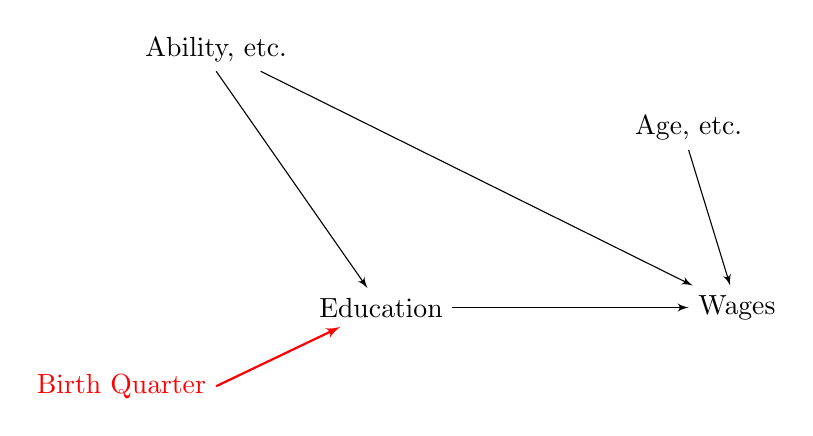
\begin{tikzpicture}[>=latex',circ/.style={draw, shape=circle, node distance=5cm, line width=1.5pt}]
		\draw[->] (0,0) node[left] (X) {Education} -- (3,0) node[right] (Y) {Wages};
		\draw[->] (-3,3) node[above] (Z) {Ability, etc.} -- (X);
		\draw[->] (Z) -- (Y);
		\draw[->] (3,2) node[above] (A) {Age, etc.} -- (Y);
		\draw<2>[->,red,thick] (-3,-1) node[left] (B) {\color{red}{Birth Quarter}} -- (X);
		\end{tikzpicture}
	\end{center}
}

\frame{
	\frametitle{How IV Works I}
	\begin{itemize}\itemsep1em
		\item Start with case where $B$ is a 0,1 indicator
		\item To identify the effect $X \rightarrow Y$, all we need is $B$
		\item We don't need to worry about other omitted variables, because the as-if-random instrument is doing all the heavy lifting for us
		\item But we don't learn anything about the rest of the causal graph
	\end{itemize}
}

\frame{
	\frametitle{How IV Works II}
	\begin{itemize}\itemsep1em
		\item Imagine two effects:
		\begin{align}
		ITT_y & = E[y_i | b_i = 1] - E[y_i | b_i = 0]\\
		ITT_x & = E[x_i | b_i = 1] - E[x_i | b_i = 0]
		\end{align}
		\item IV estimates the LATE: $\dfrac{ITT_y}{ITT_x}$
		\item In a regression, this is:\\
			$E[y_i|b_i] = \beta_0 + \text{LATE} \times E[x_i|b_i]$
		\item We can generalize this beyond an indicator IV
	\end{itemize}
}

\frame{
	\frametitle{How IV Works III}
	\begin{itemize}
		\item 
	\end{itemize}
}


\frame{
	\frametitle{}
	\begin{itemize}
	\item But, this is effect is \textit{local} to the variation in $X$ that is due to variation $B$
		\begin{itemize}
		\item Thus, IV estimation does not yield the SATE, but the LATE
		\end{itemize}
	\item 
	\end{itemize}
}



\frame{
	\frametitle{Finding Instruments}
	\begin{itemize}\itemsep1em
		\item Forward, not backward, causal inference
		\item Most instruments are not things we care about
			\begin{itemize}
				\item Weather, disasters
				\item Geography, climate
				\item Lotteries
			\end{itemize}
		\item A good instrument is one that satisfies both of our conditions, so we need:
			\begin{itemize}
				\item A good story about exogeneity
				\item Evidence that instrument is \textit{strong}
			\end{itemize}
	\end{itemize}
}

\frame{
	\frametitle{Instrumental Variables Activity}
	\begin{itemize}\itemsep2em
		\item Read each scenario
		\item Assess \textbf{exogeneity} and \textbf{relevance}
		\item Discuss with the person sitting next to you
	\end{itemize}
}


% IV estimation
% Wald
% TSLS

% LATE, SATE, and ITT


\frame{
	\frametitle{Standard Errors in IV}
	\begin{itemize}\itemsep2em
	\item SEs are larger in IV than OLS
	\item Second-stage can use ``robust'' SEs to account for heteroskedasticity
	\item The weaker the instrument, the larger the SEs
	\end{itemize}
}



% * full first stage results
% ivregress 2sls outcome covariates (confounded = instrument), first
% * additional first stage fit statistics
% estat firststage

%  Durbin-Wu-Hausman Test
% Do residuals from the first stage relate to the outcome?
% `\( Y = \beta_0 + \beta_1 X_{Confounded} + \beta_2 \nu + \epsilon\)`
% `\( \nu \)` are the residuals from the first stage

% In Stata:
% quietly ivregress 2sls outcome covariates (confounded = instrument)
% estat endogenous


% multiple instruments (overidentifying assumptions)



\section[RDD]{Regression Discontinuity Designs}
\frame{\tableofcontents[currentsection]}

\frame{
	\frametitle{Example: Maimonides' Rule}
	\begin{enumerate}\itemsep2em
		\item<2-> What is Maimonides' Rule?
		\item<3-> Why is it a valid (credible) instrument? (Or why isn't it?)
		\item<4-> How does it differ from a randomized experiment?
	\end{enumerate}
}

\frame{
	\begin{center}
		\begin{tikzpicture}[>=latex',circ/.style={draw, shape=circle, node distance=5cm, line width=1.5pt}]
		\draw[->] (0,0) node[left] (X) {Class Size} -- (3,0) node[right] (Y) {Test Scores};
		\draw[->] (-2,3) node[above] (Z) {Z} -- (X);
		\draw[->] (Z) -- (Y);
		\draw[->,red,thick] (-2,-2) node[left] (B) {\color{red}{Grade Size}} -- (X);
		\end{tikzpicture}
	\end{center}
}



\frame{
	\frametitle{How RDD Works}
	\begin{enumerate}\itemsep1em
	\item Find a consequential threshold
		\begin{itemize}
		\item Examples?
		\end{itemize}
	\item Causal inference is about comparisons
		\begin{itemize}
		\item In an experiment, $X$ is randomly assigned
		\item In matching or regression, we compare units that differ only in $X$ but are similar in $Z$
		\end{itemize}
	\item In RDD, $X$ is not randomly assigned and there is no \textit{covariate overlap}
		\begin{itemize}
		\item $B$ causally determines $X$, so units with different values of $X$ also differ in their value of $B$
		\item compare units that are as similar as possible (bandwidths)
		\end{itemize}
	\end{enumerate}
}

\frame{
	\frametitle{``Sharp'' and ``Fuzzy'' discontinuities}
	\begin{itemize}\itemsep2em
		\item If a threshold perfectly causes $X$, then it produces a \textbf{sharp} discontinuity
			\begin{itemize}
			\item Potentially analyze as an experiment
			\end{itemize}
		\item If a threshold imperfectly (probabilistically) causes $X$, then it produces a \textbf{fuzzy} discontinuity
			\begin{itemize}
			\item Analyze using Instrumental Variables
			\end{itemize}
	\end{itemize}
}


% RDD figure

\frame{
	\frametitle{Sharp RDD}
}

\frame{
	\frametitle{Fuzzy RDD}
}




\frame{
	\frametitle{Problems with Discontinuities}
	\begin{itemize}\itemsep1em
		\item Discontinuities that appear random are exploitable
		\item Compensatory rivalry and equalization
		\item Campbell's Law:\\
		\textit{The more any quantitative social indicator (or even some qualitative indicator) is used for social decision-making, the more subject it will be to corruption pressures and the more apt it will be to distort and corrupt the social processes it is intended to monitor.}
	\end{itemize}
}


\section[ITS]{Interrupted Time-Series}
\frame{\tableofcontents[currentsection]}


\frame{
	\frametitle{How ITS Works}
	\begin{itemize}\itemsep0.5em
		\item Identify an exogenous shock in $X$ that might affect $Y$
		\item Look at $Y$ before ($t$) and after ($t+1$) the shock
		\item We only observe one manifest outcome at each point in time
		\item To make a causal inference, we need:
			\begin{itemize}
				\item $Y_{0,t}$ and $Y_{1,t}$, or
				\item $Y_{0,t+1}$ and $Y_{1,t+1}$
			\end{itemize}
		\item Use pre-post comparisons to infer the value of unobserved potential outcomes		
	\end{itemize}
}



% graph over-time

\frame{
	\begin{center}
	\begin{tikzpicture}[scale=0.6]
    \draw[->] (0,0) -- (12,0) node[right] (xaxis) {};
    \draw[->] (0,0) -- (0,12) node[left] (yaxis) {};
    % x ticks
    \foreach \x in {1,2,...,11}
       	\draw (\x,1pt) -- (\x,-3pt) node[anchor=north] {};
    % y ticks
    \foreach \y in {0,...,11}
         \draw (1pt,\y) -- (-3pt,\y) node[anchor=east] {};
    % intervention
    \draw (6.5,-0.25) node[below, scale=0.5] (IV) {Intervention};
    \draw (6.5,0) -- (6.5,12);

	\draw<2-> (2,4) -- (3,2);
	\draw<2-> (3,2) -- (4,5);
	\draw<2-> (4,5) -- (5,3);
	\draw<2-> (5,3) -- (6,10);
	\draw[dashed] (6,10) -- (7,7);
	\draw<2-> (7,7) -- (8,6);
	\draw<2-> (8,6) -- (9,6);
	\draw<2-> (9,6) -- (10,4)
	\draw<2-> (10,4) -- (11,3);
	\end{tikzpicture}
	\end{center}
}




\section[DID]{Difference-In-Differences}
\frame{\tableofcontents[currentsection]}


\frame{
	\frametitle{Problem with Inference in ITS}
	\begin{itemize}\itemsep1em
		\item ITS compares a unit against itself at various points in time (pre- and post-treatment)
		\item This requires a strong assumption that potential outcomes are constant over-time:
			\begin{align*}
			Y_{i0t} \equiv Y_{i0t+1}\\
			Y_{i1t} \equiv Y_{i1t+1}
			\end{align*}
		\item If anything else changed before and after the interruption, then the shock might:
			\begin{itemize}
				\item not have been exogenous, or 
				\item have been concurrent with another change, or
				\item reflect a time trend
			\end{itemize}
	\end{itemize}
}


\frame{
	\frametitle{Difference-In-Differences}
	\begin{itemize}\itemsep1em
		\item How do we know change in $Y$ wasn't due to something else?
			\begin{itemize}
				\item How do we know $Y_{0,t}$ is a good stand-in for $Y_{0,t+1}$?
			\end{itemize}
		\item<2-> Use a comparison case (or cases)!
		\item<3-> Instead of using the pre-post difference in $Y_i$ to estimate the causal effect, use the difference in pre-post differences for two units $i$ and $j$:
		\begin{align*}
		(Y_{i,t+1} - Y_{i,t}) - (Y_{j,t+1} - Y_{j,t})
		\end{align*}
	\end{itemize}
}


\frame{
	\begin{center}
	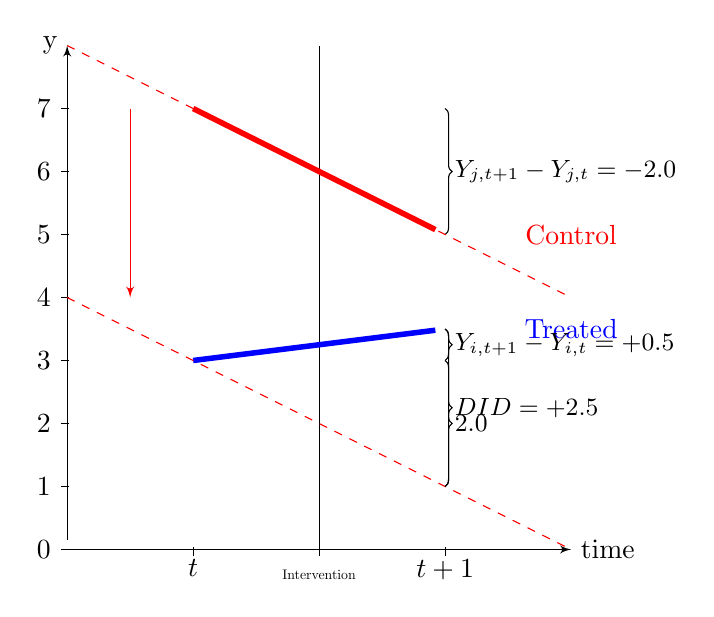
\begin{tikzpicture}[>=latex', scale=0.8]
        \draw[->] (0,0) node (origin) {}  -- (8,0) node[right] (xaxis) {time};
        \draw[->] (origin) -- (0,8) node[left] (yaxis) {y};
        % x ticks
        \foreach \x in {2,4,6}
        	\draw (\x,1pt) -- (\x,-3pt) node[anchor=north] {};
        \draw (2,0) node[below] (before) {$t$};
        \draw (6,0) node[below] (after) {$t+1$};
        \draw (4,-0.25) node[below, scale=0.5] (IV) {Intervention};
        % y ticks
        \foreach \y in {0,...,7}
             \draw (1pt,\y) -- (-3pt,\y) node[anchor=east] {$\y$};
        % intervention
        \draw (4,0) -- (4,8);

        % line
        \draw<2-> (6,3.5) node (tr) {};
        \draw<3-> (6,5) node (ctrl) {};
        \draw<2-3>[blue] (8,3.5) node (trlab) {Treated};
        \draw<3-3>[red] (8,5) node (ctrllab) {Control};        
        \draw<2->[blue, line width=2pt] (2,3) -- (tr);
        \draw<3->[red, line width=2pt] (2,7) -- (ctrl);
        
        % diffs
        \draw<4-6>[right,decorate,decoration={brace,mirror}] 
        	(6,3) -- (6,3.5) node[right, pos=0.5] (idiff) {\small $Y_{i,t+1} - Y_{i,t} = +0.5$};
        \draw<4-6>[right,decorate,decoration={brace}] 
            (6,7) -- (6,5) node[right, pos=0.5] (jdiff) {\small $Y_{j,t+1} - Y_{j,t} = -2.0$};
        
        % trends
        \draw<5-6>[red,->] (1,7) -- (1,4);
        \draw<5->[red, dashed] (0,8) -- (8,4);
        \draw<5->[red, dashed] (0,4) -- (8,0);
        \draw<6>[right,decorate,decoration={brace}] 
            (6,3) -- (6,1) node[right, pos=0.5] (idiff2) {\small $2.0$};
        \draw<7>[right,decorate,decoration={brace}] 
            (6,3.5) -- (6,1) node[right, pos=0.5] (idiff2) {\small $DID = +2.5$};
                        
        
    \end{tikzpicture}
    \end{center}
}


\frame{
	\frametitle{Causal Inference Over-Time}
	\begin{itemize}\itemsep0.5em
		\item In experiments, matching, cross-sectional regression, and RDD, we make causal inferences based on \textbf{between-unit} comparisons at the \textit{same} point in time
		\item In ITS, DID, and panel analysis (next week), we make causal inferences (also) based on \textbf{within-unit} comparisons at \textit{different} points in time
		\item This can be really helpful, but also raises new concerns
		\item We'll discuss those next week
	\end{itemize}
}



\appendix
\frame{}

\end{document}
